\section{Personalized Short-term Multi-Modal Interactions}

As already mentioned, 
one of the main goals of the COACHES project is personalized short-term multi-modal interactions with non-expert users, that are typical customers of a shopping mall.

In this context, \emph{Personalized} means that the robot should use different forms of interactions to communicate the same concept with different users, in order to increase its social acceptability;
\emph{Short-term} means that the interactions are short and focused on only one particular communicative objective, avoiding long and complex interactions; while
\emph{Multi-modality} is obtained by using different interaction devices on the robot (although in this study, we focus only on speech and graphical interfaces).



\begin{figure}
\centering
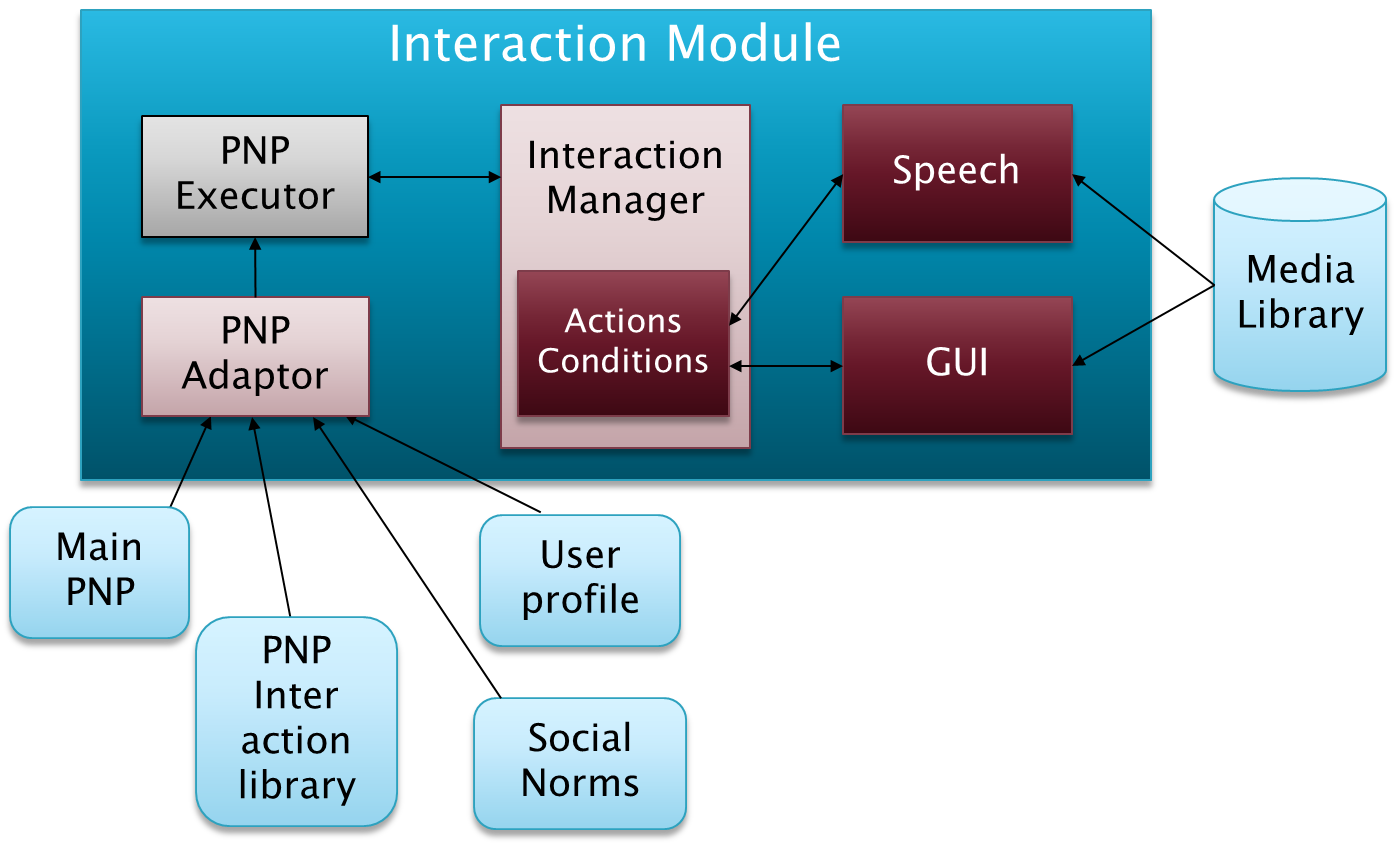
\includegraphics[width=0.95\textwidth]{fig/WP3.png}
\caption{Architecture of Interaction Module.}
\label{fig:WP3}
\end{figure}

The architecture of the Interaction Module is illustrated in Figure \ref{fig:WP3}. Data available to this module are Petri Net Plans (PNP) describing the desired behavior of the robot, User profiles and a multi-media library.

The PNPs (as described later) encode the overall behavior of the robot, as generated by the planning and reasoning components of the system. The behavior include both basic robotic actions (e.g., moving in the environment) and interaction action.

The user profile are information available about the user that is interacting with the robot. These data are in general not easy to obtain. Since this is not the focus of this paper, we assume the data are available in an appropriate format acquired with appropriate means.
Among acquisition means, it is possible to think about users wearing an RFID tag which contains personal information read by an RFID reader on-board the robot, or to the request of swiping a fidelity card, enter a personal password or showing to the robot a QR-code, in order to communicate to the robot the user profile.
In our experiments, we have used a simple identification mechanism based on recognizing QR-codes shown by the user to the robot on-board camera.

Finally, the media library is a collection of multi-media data (text, images, animations, video, etc.) that are linked to the communication activities of the robot and to the user profiles. We assume that in this library there may be different versions of the same communication item for different users. For example, ice-cream advertisement can have a different spoken text and different displayed images or videos for children and adults.

In the remaining of this section, we will describe in more details the components of the interaction module.

\subsection{PNP Adaptor and Executor}

The Interaction Module is implemented within the framework of the Petri Net Plans (PNP) formalism \cite{ZiIo}. PNPs are based on two main concepts: \emph{actions} (i.e., output operations) and \emph{conditions} (i.e., input operations). Actions include motion of the robot in the environment, spoken sentences issued by the on-board speakers, text, images, videos or animations shown on the on-board screen, etc.
Conditions include the result of perception routines (e.g., image processing or speech recognition), the input given by a user through a GUI on the on-board screen, information about personal data of user acquired through a reader of fidelity cards, etc.

The use of PNP for representing in an integrated way all these different kinds of actions and conditions allows for a strong coordination between the different sub-systems of the robot and for showing more complex behaviors and, in particular, a multi-modal interaction that can be easily customized according to the user.


The main plan, which include \emph{interaction plans} for HRI behaviors, generated by the reasoning and planning sub-system, is first processed by the PNP Adaptor and then executed by the PNP Executor. Both these modules are general-purpose, since all the relevant information are provided by external sources with an explicit representation. More specifically, the PNP Adaptor generates a personalized plan, given a main plan, a library of interaction plans, a set of social norms, and the user profile.
The generated personalized plan in then executed by the PNP Executor.

PNP Adaptor ...



PNP Executor ...




\subsection{Interaction Manager}
% Description of the Interaction Manager component...

The interactions are coordinated by an Interaction Manager (IM), which coordinates all the robot activities (both the ones related with human-robot interaction and the ones used for implementing the basic robotic functionalities).
Its goal is thus to provide effective robot behaviors, including the personalized short-term multi-modal interactions described in this section.

The IM is an action and condition server that executes actions and provides conditions, according to the requests of the PNP Executor module. It thus includes the definition of a set of primitive actions and conditions that are activated according to the plan under execution.
For the interaction behavior, actions and conditions are actually related to the Speech and Graphical Interface (GUI) modules described later. While the actions and the conditions related to the basic robot abilities (such as navigation, localization, perception, etc.) are not illustrate and described here, since the focus of this paper is on interaction.


\subsection{Speech and Graphical Interfaces}

The interaction modalities considered so far in the project are speech and graphical interfaces.


\paragraph{Speech recognition and synthesis.}
The speech component allows the robot to communicate with humans through vocal interactions. 
It is formed by Automatic Speech Recognition (ASR) and Text-To-Speech (TTS).

The ASR component analyzes audio data coming from a microphone and extract semantic information about the spoken sentences, according to a predefined grammar. This component allows the robot to understand user spoken commands.
The speech recognition module is based on the Microsoft engine and on a further processing module that builds the semantic frames of the recognized sentences.
More details on the approach are available in \cite{Ba...}.

The TTS component transforms text messages in audio data that are then emitted by the speakers on-board the robot. This enables the robot to speak to people. The Microsoft TTS engine is used for this module.


\paragraph{Graphical User Interface.}

The GUI component implements a graphical input and output interface between users and robots that is displayed through the touch screen on-board the robot. The GUI defines actions (i.e., output operations) and conditions (i.e., input operations) that are integrated in the IM with other communication primitives (e.g., speech) in order to implement a multi-modal interaction.

\vspace{1cm}

The Speech and GUI components make available to the IM the implementation of actions and conditions that are executed according to the PNPs. These are summarized in the following table.

\vspace{1em}
\begin{center}
%\begin{table}
\begin{tabular}{|c|c|c|} \hline
 & {\bf Action} & {\bf Condition} \\  \hline
Speech & 
\begin{tabular}{c}
\emph{Say} \\ 
speak information though TTS
\end{tabular} & 
\begin{tabular}{c}
\emph{ASR} \\ 
Results of ASR
\end{tabular} \\ \hline
GUI & 
\begin{tabular}{c}
\emph{Show} \\ 
show information on the GUI
\end{tabular} & 
\begin{tabular}{c}
\emph{GUI} \\ 
Results of GUI input
\end{tabular} \\ \hline
\end{tabular}  
%\label{}
%\caption
\end{center}
\vspace{1em}


